\section{Zeta funkcije grafov in Riemannova hipoteza}
Večina praktičnih uporab Ramanujanovih grafov pravzaprav ne zahteva, da so grafi točno Ramanujanovi. Običajno imamo nek postopek za katerega velja, da če je naš graf bolje povezan (oziroma, da je druga največja lastna vrednost čim manjša), bomo dobili boljše rezultate. Velja sicer, da so Ramanujanovi grafi optimalni glede na ta kriterij, torej bi pri njih dobili najboljše rezultate, niso pa strogo potrebni. Želimo pa si ogledati primer uporabe ali lastnosti Ramanujanovih grafov, kjer bi bilo zares ključno, da so grafi Ramanujanovi. Zato si bomo ogledali eno izmed najpomembnejših domnev v matematiki, Riemannovo hipotezo. Ta opisuje obnašanje ničel določene kompleksne funkcije, vendar se izkaže, da obstaja analog te funkcije na grafih; vsakemu regularnemu grafu pripada neka kompleksna funkcija. Izrek bomo natančno formulirali kasneje, vendar pa dokaza običajne Riemannove hipoteze še ne poznamo. Zanimivo pa je, da je za različico z grafi dokaz že znan: izkaže se, da funkcija, ki pripada grafu, zadošča Riemannovi hipotezi natanko takrat, ko je graf Ramanujanov \cite{portablesnowbird}.

\subsection{Riemannova zeta funkcija}
Začeli bomo z običajno Riemannovo zeta funkcijo \cite{freitag1}. Enostavno jo je definirati kot analitično funkcijo na \(\Re(z)>1\) z
\begin{align*}
    \zeta(z) &= \sum_{n=1}^\infty \frac{1}{n^z} \\ 
    &= \prod_{p \text{ praštevilo}} \left(1-p^{-z}\right)^{-1}.
\end{align*}
Funkcijo \((1-z)\zeta(z)\) lahko analitično razširimo na celotno kompleksno ravnino, torej lahko tudi \(\zeta\) razširimo v meromorfno funkcijo na \(\C\) s polom v \(z=1\). Že iz alternativnega zapisa funkcije vidimo, da je tesno povezana s praštevili, Riemann pa je razširjeno različico uporabil, da je dokazal praštevilski izrek, ki pravi, da število praštevil manjših od števila \(n\) asimptotsko raste z \(\frac{n}{\log{n}}\). Ničle \(\zeta\) funkcije pa nam o tem izreku lahko povejo še več, z njimi lahko opišemo napako v oceni iz praštevilskega izreka in s tem bolje razumemo porazdelitev praštevil.

Ničle Riemannove zeta funkcije delimo na trivialne in na netrivialne. Najprej si oglejmo trivialne ničle ter območja, kjer je enostavno videti, da funkcija nima ničel. Nerazširjena zeta funkcija (torej na vrednostih \(\Re(z) > 1\)) nima ničel. Praštevilski izrek je ekvivalenten temu, da na premici \(\Re(z) = 1\) ni ničel \cite{harolddiamond}. Za negativno polravnino (\(\Re(z) \leq 0\)) je enostavno poiskati ničle, tu dobimo \emph{trivialne ničle}, ki se nahajajo v točkah \(-2k\) za \(k\in\Z^+\). Drugih ničel na tej polravnini ni.

Ostane nam samo še množica \(\{z\in \C\mid 0 < \Re(z) < 1\}\), ki jo imenujemo kritični trak. Tu se nahajajo netrivialne ničle, točne distribucije pa ne poznamo. Znotraj traka se nahaja kritična premica \(\{z\in \C \mid \Re(z) = 1/2\}\). Znano je, da se na tej premici nahaja več kot 40\% netrivialnih ničel \cite{Pratt2019}. Računsko smo izračunali že vsaj 100 milijard ničel zeta funkcije na kritičnem traku in vse so na kritični premici \cite{racunskoniclezeta}. To nas pripelje do Riemannove hipoteze.

\begin{izrek}[Riemannova hipoteza]
    Vse netrivialne ničle zeta funkcije se nahajajo na kritični premici.
\end{izrek}

\subsection{Ihara zeta funkcija}
Sedaj bomo definirali zeta funkcijo, ki pripada grafu. Definicija te funkcije bo analogna definiciji klasične zeta funkcije, še bolj pa je sorodna Selbergovi zeta funkciji, ki si je ne bomo ogledali \cite{sunada-zetagrafov}.

Z \(s=(v_0, \ldots, v_{l})\) označimo sklenjen okrajšan sprehod v grafu. To je sprehod, ki ne obišče dveh vozlišč zaporedoma (torej \(v_i \neq v_{i+2}\), kot v definiciji \ref{okrajsana-beseda}), začne in konča pa se v istem vozlišču (torej \(v_0 = v_l\)). Z \(L(s)=l\) označimo dolžino takega sprehoda. Bolj kot zaporedje vozlišč nas zanima oblika poti v grafu neodvisno od začetne točke. Če dodamo še zahtevo \(v_1 \neq v_{l-1}\), lahko obravnavamo vse take sprehode kot ekvivalentne (torej dva sprehoda sta ekvivalentna, če se zaporedje vozlišč razlikuje za ciklično permutacijo). To nam definira pojem zaprte geodezijke v grafu. 

\begin{definicija}[Zaprta geodezijka grafa]
    Zaprta geodezijka grafa je ekvivalenčni razred sprehodov \(s\) dolžine \(l\), za katere velja
    \begin{align*}
        v_0 = v_l \\
        v_i \neq v_{i+2 \pmod l},
    \end{align*}
    dva sprehoda \(s=(v_0, \ldots, v_{l})\) in \(s'=(v_0', \ldots, v_{l}')\) pa sta si ekvivalentna, če obstaja ciklična permutacija \(\pi\) na \(\{0, \ldots, l-1\}\), za katero velja \(v_{\pi(i)} = v_i'\) za vsak \(i\). 
\end{definicija}

Če geodezijke ne moremo dobiti tako, da večkrat ponovimo krajšo pot, je ta geodezijka nerazcepna. Na primer, v 3-ciklu nam pot \((v_0, v_1, v_2, v_0)\) definira zaprto nerazcepno geodezijko, pot \((v_0, v_1, v_2, v_0, v_1, v_2, v_0)\) pa zaprto razcepno geodezijko. Namesto praštevil v definiciji zeta funkcije bomo iterirali po nerazcepnih geodezijkah, množico le-teh pa označimo z \(P\).

\begin{definicija}[Ihara zeta funkcija]
    Ihara zeta funkcija grafa \(G\) je analitično nadaljevanje funkcije
    \begin{align*}
        \zeta_G(z) = \prod_{p\in P}\left(1-z^{L(p)}\right)^{-1}.
    \end{align*}
\end{definicija}
 
Z \(\alpha_G\) označimo konvergenčni radij vrste. Za \(d\)-regularne grafe je ta enak kar \(\alpha_G = 1/(d-1)\), Ihara zeta funkcija pa je racionalna funkcija. V primeru regularnih grafov lahko funkcijo opišemo še bolje: izkaže se namreč, da je recipročna funkcija \(\zeta_G^{-1}\) cela funkcija, torej \(\zeta_G\) nima ničel. Od tu naprej bodo vsi grafi regularni.

% https://en.wikipedia.org/wiki/Ihara_zeta_function#cite_note-2
% Portable snowbird
% https://drops.dagstuhl.de/storage/00lipics/lipics-vol093-fsttcs2017/LIPIcs.FSTTCS.2017.46/LIPIcs.FSTTCS.2017.46.pdf
\begin{izrek}[Bassova formula Ihara zeta funkcije]\label{zeta-je-racionalna-bass}
    Za \(d\)-regularen graf \(G\) z \(n\) vozlišči in \(m=d\cdot n / 2\) povezavami je njegova Ihara zeta funkcija enaka
    \begin{align*}
        \zeta_G(z) = \left((1-z^2)^{m-n}\det(I-Az+(d-1)z^2I)\right)^{-1}.
    \end{align*}
\end{izrek}
Ogledali si bomo dokaz izreka Bassove formule \cite{rangarajan:LIPIcs.FSTTCS.2017.46}, najprej pa potrebujemo še nekaj pomožnih pojmov. Potence sosednostne matrike nam opisujejo število poti. Kot smo že uporabili v prejšnjih poglavjih (na primer v izreku \ref{alon-boppanova-meja-izrek}), nam sled matrike \(A^k\) da število ciklov dolžine \(k\) v grafu. Podobno lahko izračunamo tudi število geodezijk, le da namesto sosednostne matrike uporabimo Hashimotovo matriko.
\begin{definicija}[Hashimotova matrika]
    Hashimotova matrika za \(d\)-regularen graf \(G\) na \(n\) vozliščih je \(\C^{dn\times dn}\) matrika. Elementi te matrike opisujejo obstoj poti brez povračanja. Če imamo urejena para \(e_1 = (u, v)\) in \(e_2= (u', v')\), potem je \(H_{e_1, e_2}=1\), če \(v = u'\) (pot iz \(e_1\) vodi v \(e_2\)) in \(u\neq v'\) (pot je brez povračanja). Vsi ostali elementi so ničelni.
\end{definicija}
\begin{primer}{Hashimotova matrika cikla}
    Oglejmo si Hashimotovo matriko \(3\)-cikla. Sosednostna matrika cikla je
    \begin{align*}
        \begin{bmatrix}
            0&1&1\\
            1&0&1\\
            1&1&0
        \end{bmatrix}.
    \end{align*}
    Če njegove povezave uredimo kot \((1,2), (1,3), (2,1), (2,3), (3,1), (3,2)\), potem je njegova Hashimotova matrika enaka
    \begin{align*}
        H = \begin{bmatrix}
            0&0&0&1&0&0\\
            0&0&0&0&0&1\\
            0&1&0&0&0&0\\
            0&0&0&0&1&0\\
            1&0&0&0&0&0\\
            0&0&1&0&0&0
        \end{bmatrix}.
    \end{align*}
    Sled te matrike je enaka \(0\), prav tako je tudi sled matrike \(H^2\) enaka 0. Matrika \(H^3\) pa je enaka identični matriki, torej je njena sled enaka \(6\). To predstavlja tri cikle v smeri urinega kazalca (eno za vsako začetno vozlišče) in tri cikle v obratni smeri, iz česar dobimo dve geodezijki dolžine tri. 
\end{primer}
Matrika ni nujno simetrična. Če z \(\tilde{n}_k\) označimo število ciklov brez povračanja, potem \(\tilde{n}_k = \Tr(H^k)\), podobno kot analogna lastnost pri sosednostni matriki. Vsako razcepno geodezijko lahko dobimo tako, da neko nerazcepno geodezijko večkrat ponovimo. Torej velja
\begin{align}\label{enakost-l-tilden}
    \sum_{k=1}^\infty \tilde{n}_k \frac{z^k}{k} = \sum_{p\in P} L(p)\left(\sum_{m=1}^\infty \frac{z^{mL(p)}}{mL(p)}\right),
\end{align}
saj v vsoti na levi iteriramo po vseh geodezijkah, na vsoti na desni pa najprej po vseh nerazcepnih geodezijkah, nato pa vseh njihovih ponovitvah. Dobili smo še faktor \(L(p)\), saj en ekvivalenčni razred lahko dobimo na \(L(p)\) načinov (saj lahko začnemo šteti na kateri koli točki cikla). Z ugotovljenim lahko dokažemo naslednjo lemo.

\begin{lema}[Hashimotova formula Ihara zeta funkcije]
    Za graf \(G\) in njegovo Hashimotovo matriko \(H\) velja
    \begin{align*}
        \zeta_G(z) = \det(I-Hz)^{-1}.
    \end{align*}
\end{lema}
\begin{dokaz}
    Razpišemo zeta funkcijo po definiciji.
    \begin{align*}
        \zeta_G(z) &= \prod_{p\in P}\frac{1}{1-z^{L(p)}} \\
        &= \exp\left(-\sum_{p\in P}\log(1-z^{L(p)})\right)
    \end{align*}
    Notranjo vrsto lahko po Taylorju razvijemo
    \begin{align*}
        \zeta_G(z) =\exp\left(\sum_{p\in P}\sum_{m=1}^\infty \frac{z^{L(p)m}}{m}\right),
    \end{align*}
    nato pa uporabimo enakost \ref{enakost-l-tilden}.
    \begin{align*}
        \zeta_G(z) =\exp\left(\sum_{k=1}^\infty \tilde{n}_k \frac{z^k}{k}\right)
    \end{align*}
    V ta izraz lahko enostavno vpeljemo Hashimotovo matriko.
    \begin{align*}
        \zeta_G(z) &= \exp\left(\sum_{k=1}^\infty \Tr(H^k)\frac{z^k}{k}\right)\\
        &= \exp\left(-\Tr(\log(I - zH))\right)
    \end{align*}

    Po Jacobijevi formula velja \(\det A = \exp \Tr(\log A)\), torej izraz lahko preoblikujemo v
    \begin{align*}
        \zeta_G(z) = \det(I-zH)^{-1}.
    \end{align*}
\end{dokaz}
Dobljeni izraz je že dovolj, da vidimo, da je \(\zeta_G^{-1}\) pravzaprav cela funkcija. Dokaz Bassove formule (\ref{zeta-je-racionalna-bass}) je od tu naprej le računski, zato orišemo le skico postopka. Omenimo pa še, da se da Bassovo formulo dokazati tudi drugače, in sicer s pomočjo polinomov Čebiševa. Opazimo lahko namreč, da je izraz v formuli zelo podoben generatorski funkciji polinomov Čebiševa.

\begin{dokaz}[Skica dokaza Bassove formule]
    Definiramo \(n\times dn\) matriko \(S\), \(dn \times n\) matriko \(T\) in \(dn \times dn\) matriko \(B\).
    \begin{align*}
        S_{w, (u, v)} &= \begin{cases}
            1 & u = w\\
            0 & \text{sicer}
        \end{cases}\\
        T_{(u, v), w} &= \begin{cases}
            1 & v = w\\
            0 & \text{sicer}
        \end{cases}\\
        B_{(u, v), (u', v')} &= \begin{cases}
            1 & v = u' \text{ in } v' = u\\
            0 & \text{sicer}
        \end{cases}
    \end{align*}
    Za te matrike veljajo relacije
    \begin{align*}
        A = ST, \\ 
        H = TS - B, \\
        SBT = dI.
    \end{align*}
    Te relacije povezujejo matriki \(A\) in \(H\), preostanek dokaza pa je le računski.
\end{dokaz}

\subsection{Riemannova hipoteza}

Zdaj poznamo strukturo Ihara zeta funkcije grafa in si lahko podrobneje ogledamo njene lastnosti. Ker funkcija nima ničel, si bomo namesto njih ogledali pole (oziroma ničle funkcije \(\zeta_G^{-1}\)). Če ima graf \(m\) povezav, je teh polov \(2m\), kot vidimo iz Hashimotove formule, saj je \(H\) dimenzije \(2m\times 2m\). Podobno kot pri ničlah zeta funkcije se tudi poli Ihara zeta funkcije nahajajo le na določenem delu kompleksne ravnine. Če je \(\lambda\) pol \(\zeta_G\), potem je \((d-1)^{-1}\leq \abs{\lambda}\leq 1\). Pola \((d-1)^{-1}\) in \(1\) ustrezata največji lastni vrednosti regularnih grafov, \(d\). Taki poli na robu območja so trivialni, preostali pa netrivialni. To definira različico kritičnega traku za Ihara zeta funkcijo, kritična premica pa ustreza krožnici \(\abs{\lambda}=\sqrt{d-1}^{-1}\). Riemannova hipoteza v tem primeru pravi, da če je \(\lambda\) netrivialen pol \(\zeta_G\), potem \(\abs{\lambda} = \sqrt{d-1}^{-1}\). Ta hipoteza velja natanko takrat, ko je graf \(G\) Ramanujanov \cite{murty-notintro}.

\begin{izrek}[Riemannova hipoteza za grafe]
    Za \(d\)-regularen graf \(G\) velja, da je Ramanujanov natanko takrat, ko za vsak netrivialen pol \(\lambda\in\C\) njegove Ihara zeta funkcije \(\zeta_G\) velja
    \begin{align*}
        \abs{\lambda} = \frac{1}{\sqrt{d-1}}.
    \end{align*}
\end{izrek}
\begin{dokaz}
    Zeta funkcijo najprej zapišemo v Bassovi obliki, kot v izreku \ref{zeta-je-racionalna-bass}.
    \begin{align*}
        \zeta_G(z) = \left((1-z^2)^{m-n}\det(I-Az+(d-1)z^2I)\right)^{-1}.
    \end{align*}
    Zapišemo še karakteristični polinom grafa \(G\):
    \begin{align*}
        \chi_G(\lambda ) = \det(\lambda I-A).
    \end{align*}
    Če uporabimo substitucijo \(\lambda = (1+(d-1)z^2)/z\), potem dobimo
    \begin{align*}
        &\det\left(\frac{(1+(d-1)z^2)}{z} I - A\right)\\
        =& z^{-n}\det\left((1+(d-1)z^2) I - zA\right) \\
        =& z^{-n}\det\left(I-Az+(d-1)z^2I\right) 
    \end{align*}
    Torej poli \(\zeta_G\) izvirajo iz ničel polinoma \(\chi_G\) oziroma iz lastnih vrednosti grafa \(G\).

    Dokažimo najprej implikacijo v desno, torej predpostavimo, da je \(G\) Ramanujanov graf. Za vsako njegovo netrivialno lastno vrednost\(\lambda_0\) velja \(\abs{\lambda_0} \leq 2\sqrt{d-1}\) in zato tudi \(\lambda_0^2 \leq 4(d-1)\). Prepišemo substitucijo \(\lambda\) od zgoraj v standardno obliko.
    \begin{align*}
        \lambda = (1+(d-1)z^2)/z \\
        (d-1)z^2 - \lambda z + 1 = 0
    \end{align*}
    in tako dobimo
    \begin{align*}
        z_0 = \frac{\lambda_0 \pm \sqrt{\lambda_0^2-4(d-1)}}{2(d-1)}.
    \end{align*}
    Ker je \(\lambda_0^2-4(d-1)\leq 0\), potem je \(z_0\) enak \(\pm 1/\sqrt{d-1}\), ali pa ni realen. V prvem primeru smo končali, saj smo dobili pol na kritični premici. V nasprotnem primeru pa vstavimo dobljeni pol \(z_0\) v substitucijo.
    \begin{align*}
        \lambda_0 &= \frac{\lambda_0 \overline{z_0}}{\overline{z_0}}\\
        &= \frac{(1+(d-1)z_0^2)\overline{z_0}}{z_0\overline{z_0}}\\
        &= \frac{\overline{z_0} + (d-1)\abs{z_0}^2z_0}{\abs{z_0}^2}
    \end{align*}
    Imaginarni del izraza v imenovalcu je enak \(-\Im(z_0) + (d-1)\abs{z_0}^2\Im(z_0)\). Vse lastne vrednosti grafa, vključno z izbrano \(\lambda_0\), so realne, torej more biti ta imaginarni del enak nič. To pa pomeni, da je \((d-1)\abs{z_0}^2 = 1\) oziroma \(\abs{z_0} = 1/\sqrt{d-1}\), kot zahteva izrek.

    Podobno sledi tudi izrek v obratno smer. Če je \(z_0\) netrivialen pol, predpostavimo, da velja \((d-1)\abs{z_0}^2 = 1\). Podobno kot prej poračunamo \(\lambda_0\).
    \begin{align*}
        \lambda_0 &= \frac{\overline{z_0} + (d-1)\abs{z_0}^2z_0}{\abs{z_0}^2}\\
        &= (d-1)(\overline{z_0} + z_0)
    \end{align*}
    Ogledamo si absolutno vrednost:
    \begin{align*}
        \abs{\lambda_0} = (d-1)\abs{\overline{z_0} + z_0} \leq 2(d-1)\abs{z_0} = 2\sqrt{d-1}.
    \end{align*}
    To zaključi še dokaz v obratno smer.
\end{dokaz}

Če uporabimo substitucijo \(w = (d-1)^{-z}\), dobimo vrsto, ki nima polov za \(\Re(w)>1\) ter ima pol prvega reda v \(w=1\). Če to navežemo na lastne vrednosti grafov, lastnost, da ni polov z \(\Re(w)>1\) ustreza lastnosti regularnih grafov, da nimajo lastnih vrednosti večjih od \(d\). Imajo pa eno lastno vrednost enako \(d\), kar ustreza polu prvega reda v \(w=1\). Kritični trak je tako, podobno kot pri klasični Riemannovi zeta funkciji, trak \(0<\Re(w)<1\). Riemannova hipoteza za Ihara zeta funkcijo pa je analogna klasični Riemannovi hipotezi -- da imajo vse ničle, ki se nahajajo na kritičnemu traku, realno komponento enako \(1/2\).

Za konec si oglejmo še primere zeta funkcij grafov iz uvodnega poglavja.

\begin{primer}[Naključen graf]
    Vzamemo graf \(G\) iz primera \ref{nakljucen-graf-cheeger}. Ta graf je \(5\)-regularen graf na dvanajstih vozliščih. Izračunali smo že, da je Ramanujanov.

    Njegova zeta funkcija ima \(5\cdot 12 = 60\) polov. Vsi netrivialni poli so enaki \(1/\sqrt{5-1}\) po absolutni vrednosti.

    \begin{figure}[H]
        \centering
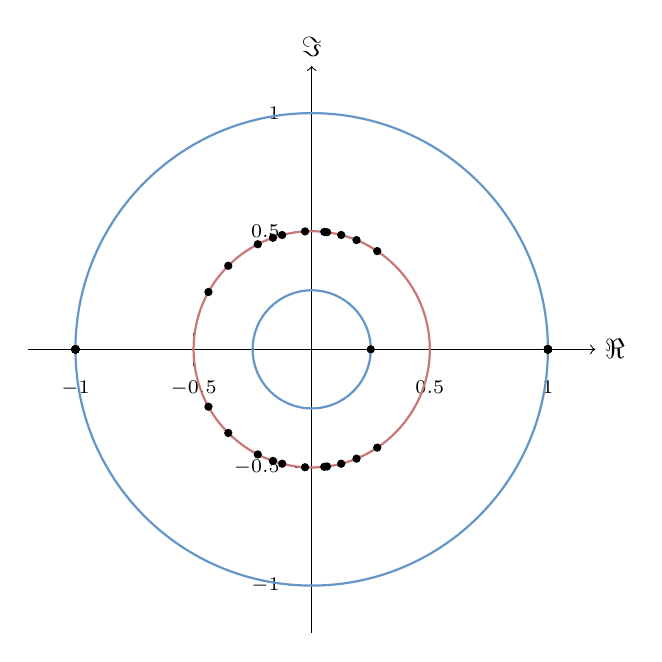
\begin{tikzpicture}[scale=3]
  % Axes
  \draw[->] (-1.2,0) -- (1.2,0) node[right] {$\Re$};
  \draw[->] (0,-1.2) -- (0,1.2) node[above] {$\Im$};
  % Ticks on x-axis
  \foreach \x in {-1,-0.5,0.5,1}
    \draw (\x,2pt) -- (\x,-2pt) node[below=2pt] {\scriptsize $\x$};
  % Ticks on y-axis
  \foreach \y in {-1,-0.5,0.5,1}
    \draw (2pt,\y) -- (-2pt,\y) node[left=2pt] {\scriptsize $\y$};
  
  \definecolor{softblue}{RGB}{100,150,200}
  \definecolor{softred} {RGB}{200,120,120}

  % Circles centered at the origin
  \draw[thick, softblue] (0,0) circle (1);    % |z| = 1
  \draw[thick, softblue] (0,0) circle (0.25); % |z| = 1/(5-1)=0.25
  \draw[thick, softred ] (0,0) circle (0.5);  % |z| = 1/sqrt(5-1)=0.5
  \fill (0.24999999999999967,0.0) circle (0.5pt);
\fill (-0.4371169307497872,-0.2427525259433682) circle (0.5pt);
\fill (-0.4371169307497872,0.2427525259433682) circle (0.5pt);
\fill (-0.35314559789735017,-0.35396071347781394) circle (0.5pt);
\fill (-0.35314559789735017,0.35396071347781394) circle (0.5pt);
\fill (0.27745431702368445,-0.41595564903595295) circle (0.5pt);
\fill (0.27745431702368445,0.41595564903595295) circle (0.5pt);
\fill (-0.22806120755953882,-0.44495852122021967) circle (0.5pt);
\fill (-0.22806120755953882,0.44495852122021967) circle (0.5pt);
\fill (0.18987905023713797,-0.46254291290759464) circle (0.5pt);
\fill (0.18987905023713797,0.46254291290759464) circle (0.5pt);
\fill (-0.16409853281752337,-0.47230463847726073) circle (0.5pt);
\fill (-0.16409853281752337,0.47230463847726073) circle (0.5pt);
\fill (-0.12499999999999986,-0.48412291827592674) circle (0.5pt);
\fill (-0.12499999999999986,0.48412291827592674) circle (0.5pt);
\fill (-0.028244530374202725,-0.49920160907587324) circle (0.5pt);
\fill (-0.028244530374202725,0.49920160907587324) circle (0.5pt);
\fill (0.1250000000000007,-0.48412291827592707) circle (0.5pt);
\fill (0.1250000000000007,0.48412291827592707) circle (0.5pt);
\fill (0.053351785269372724,-0.4971454384871406) circle (0.5pt);
\fill (0.053351785269372724,0.4971454384871406) circle (0.5pt);
\fill (0.06498164686820843,-0.4957594029065872) circle (0.5pt);
\fill (0.06498164686820843,0.4957594029065872) circle (0.5pt);
\fill (0.9999999999999991,0.0) circle (0.5pt);
\fill (1.0000000000000004,0.0) circle (0.5pt);
\fill (-0.9999999999999996,-0.0) circle (0.5pt);
\fill (-0.9999999999999996,-0.0) circle (0.5pt);
\fill (-1.0000000000000007,-0.0) circle (0.5pt);
\fill (1.0000000000000013,0.0) circle (0.5pt);
\fill (-1.0000000000000004,-0.0) circle (0.5pt);
\fill (-0.9999999999999996,-0.0) circle (0.5pt);
\fill (-1.0000000000000002,-0.0) circle (0.5pt);
\fill (1.0000000000000009,0.0) circle (0.5pt);
\fill (0.9999999999999998,0.0) circle (0.5pt);
\fill (0.9999999999999989,0.0) circle (0.5pt);
\fill (0.9999999999999998,0.0) circle (0.5pt);
\fill (1.0000000000000002,0.0) circle (0.5pt);
\fill (-0.9999999999999996,-0.0) circle (0.5pt);
\fill (-1.0,-0.0) circle (0.5pt);
\fill (0.9999999999999993,0.0) circle (0.5pt);
\fill (0.9999999999999998,0.0) circle (0.5pt);
\fill (-1.0000000000000009,-0.0) circle (0.5pt);
\fill (-1.0000000000000002,-0.0) circle (0.5pt);
\fill (0.9999999999999984,0.0) circle (0.5pt);
\fill (0.9999999999999989,0.0) circle (0.5pt);
\fill (-0.9999999999999998,-0.0) circle (0.5pt);
\fill (-1.0000000000000004,-0.0) circle (0.5pt);
\fill (-0.9999999999999998,-0.0) circle (0.5pt);
\fill (0.9999999999999993,0.0) circle (0.5pt);
\fill (1.0,0.0) circle (0.5pt);
\fill (0.9999999999999993,0.0) circle (0.5pt);
\fill (-1.0,-0.0) circle (0.5pt);
\fill (-0.9999999999999998,-0.0) circle (0.5pt);
\fill (0.9999999999999998,0.0) circle (0.5pt);
\fill (0.9999999999999989,0.0) circle (0.5pt);
\fill (-0.9999999999999991,-0.0) circle (0.5pt);
\fill (-0.9999999999999996,-0.0) circle (0.5pt);
\fill (-0.9999999999999996,-0.0) circle (0.5pt);
\fill (0.9999999999999996,0.0) circle (0.5pt);
\fill (1.0,0.0) circle (0.5pt);
\end{tikzpicture}
\caption{Poli Ihara zeta funkcije naključnega grafa.}
\end{figure}
\end{primer}
\begin{primer}[Ozko grlo]
    Oglejmo si še graf iz primera \ref{ozko-grlo-cheeger}. Za ta graf ozkega grla vemo, da ni Ramanujanov, torej njegovi poli ne smejo vsi ležati na kritični krožnici.
    \begin{figure}[H]
        \centering
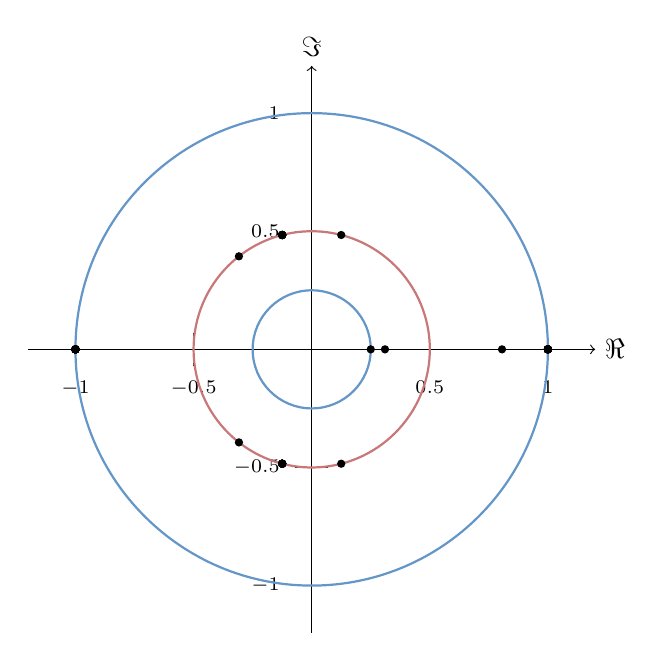
\begin{tikzpicture}[scale=3]
  % Axes
  \draw[->] (-1.2,0) -- (1.2,0) node[right] {$\Re$};
  \draw[->] (0,-1.2) -- (0,1.2) node[above] {$\Im$};
  % Ticks on x-axis
  \foreach \x in {-1,-0.5,0.5,1}
    \draw (\x,2pt) -- (\x,-2pt) node[below=2pt] {\scriptsize $\x$};
  % Ticks on y-axis
  \foreach \y in {-1,-0.5,0.5,1}
    \draw (2pt,\y) -- (-2pt,\y) node[left=2pt] {\scriptsize $\y$};
  
  \definecolor{softblue}{RGB}{100,150,200}
  \definecolor{softred} {RGB}{200,120,120}

  % Circles centered at the origin
  \draw[thick, softblue] (0,0) circle (1);    % |z| = 1
  \draw[thick, softblue] (0,0) circle (0.25); % |z| = 1/(5-1)=0.25
  \draw[thick, softred ] (0,0) circle (0.5);  % |z| = 1/sqrt(5-1)=0.5
  \fill (0.24999999999999978,0.0) circle (0.5pt);
  \fill (0.31026651025033947,0.0) circle (0.5pt);
  \fill (-0.30801270189221924,-0.3938631430751735) circle (0.5pt);
  \fill (-0.30801270189221924,0.3938631430751735) circle (0.5pt);
  \fill (0.8057588935340989,0.0) circle (0.5pt);
  \fill (0.125,-0.4841229182759273) circle (0.5pt);
  \fill (0.125,0.4841229182759273) circle (0.5pt);
  \fill (-0.1250000000000001,-0.48412291827592674) circle (0.5pt);
  \fill (-0.1250000000000001,0.48412291827592674) circle (0.5pt);
  \fill (-0.12500000000000017,-0.4841229182759272) circle (0.5pt);
  \fill (-0.12500000000000017,0.4841229182759272) circle (0.5pt);
  \fill (-0.12500000000000006,-0.48412291827592735) circle (0.5pt);
  \fill (-0.12500000000000006,0.48412291827592735) circle (0.5pt);
  \fill (-0.12500000000000008,-0.48412291827592707) circle (0.5pt);
  \fill (-0.12500000000000008,0.48412291827592707) circle (0.5pt);
  \fill (-0.12499999999999996,-0.48412291827592635) circle (0.5pt);
  \fill (-0.12499999999999996,0.48412291827592635) circle (0.5pt);
  \fill (-0.12500000000000017,-0.48412291827592707) circle (0.5pt);
  \fill (-0.12500000000000017,0.48412291827592707) circle (0.5pt);
  \fill (-0.12499999999999972,-0.48412291827592674) circle (0.5pt);
  \fill (-0.12499999999999972,0.48412291827592674) circle (0.5pt);
  \fill (-0.12499999999999957,-0.4841229182759272) circle (0.5pt);
  \fill (-0.12499999999999957,0.4841229182759272) circle (0.5pt);
  \fill (1.0000000000000002,0.0) circle (0.5pt);
  \fill (0.9999999999999996,0.0) circle (0.5pt);
  \fill (0.9999999999999978,0.0) circle (0.5pt);
  \fill (1.0,0.0) circle (0.5pt);
  \fill (1.0000000000000009,0.0) circle (0.5pt);
  \fill (-0.9999999999999991,-0.0) circle (0.5pt);
  \fill (-0.9999999999999973,-0.0) circle (0.5pt);
  \fill (-0.9999999999999993,-0.0) circle (0.5pt);
  \fill (-0.9999999999999984,-0.0) circle (0.5pt);
  \fill (-0.9999999999999987,-0.0) circle (0.5pt);
  \fill (-0.9999999999999996,-0.0) circle (0.5pt);
  \fill (-1.0000000000000004,-0.0) circle (0.5pt);
  \fill (-0.9999999999999998,-0.0) circle (0.5pt);
  \fill (0.9999999999999993,-4.299875284949252e-16) circle (0.5pt);
  \fill (0.9999999999999993,4.299875284949252e-16) circle (0.5pt);
  \fill (0.9999999999999998,0.0) circle (0.5pt);
  \fill (1.0000000000000007,0.0) circle (0.5pt);
  \fill (1.0000000000000002,0.0) circle (0.5pt);
  \fill (-0.9999999999999996,-0.0) circle (0.5pt);
  \fill (-0.9999999999999996,-0.0) circle (0.5pt);
  \fill (1.0000000000000007,0.0) circle (0.5pt);
  \fill (0.9999999999999993,0.0) circle (0.5pt);
  \fill (1.0000000000000004,0.0) circle (0.5pt);
  \fill (-1.0000000000000016,-0.0) circle (0.5pt);
  \fill (-0.9999999999999991,-0.0) circle (0.5pt);
  \fill (-1.0000000000000004,-0.0) circle (0.5pt);
  \fill (-1.0000000000000002,-0.0) circle (0.5pt);
  \fill (-0.9999999999999989,-0.0) circle (0.5pt);
  \fill (1.0000000000000007,0.0) circle (0.5pt);
  \fill (-1.0,-0.0) circle (0.5pt);
  \fill (-0.9999999999999996,-0.0) circle (0.5pt);
  \fill (-1.0000000000000009,-0.0) circle (0.5pt);
  \fill (1.0000000000000007,0.0) circle (0.5pt);
  \fill (0.9999999999999993,0.0) circle (0.5pt);
  \fill (1.0000000000000002,0.0) circle (0.5pt);
  \fill (1.0,0.0) circle (0.5pt);
  \fill (1.0000000000000009,0.0) circle (0.5pt);
\end{tikzpicture}
\caption{Poli Ihara zeta funkcije grafa ozkega grla.}
\end{figure}
\end{primer}